De veeltermbenadering van de functie van Runge $f(x,y)=\frac{1}{1+25(x^2+y^2)}$ gebruik makend van twee verschillende roosters wordt getoond in figuur~\ref{fig:oef14resultaat}.
Zowel een rooster met equidistante punten (links) als een rooster met niet-equidistante punten (rechts) werd gebruikt ter vergelijking.

\begin{figure}[H]
    \centering
    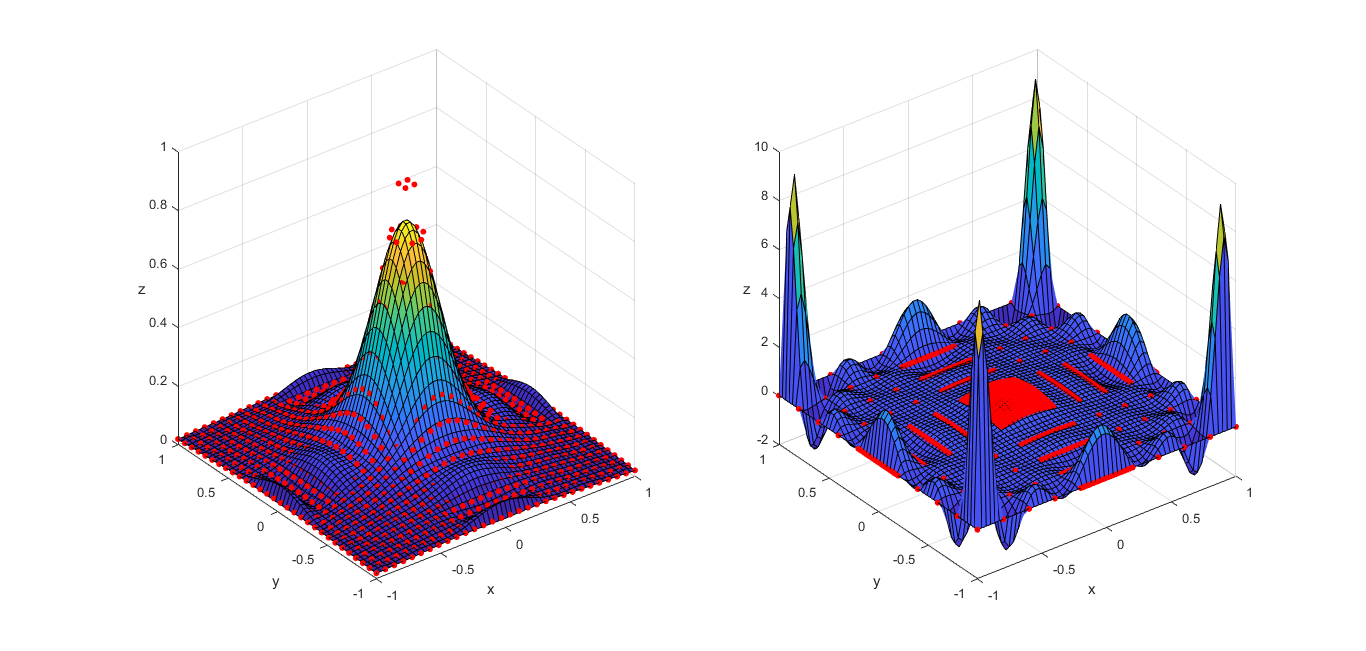
\includegraphics[width=0.8\textwidth]{oef1410.png}
    \caption{veeltermbenadering van graad $10$ in $x$ en $y$ van de functie van Runge $f(x,y)=\frac{1}{1+25(x^2+y^2)}$ gebruik makend van equidistante roosterpunten (links) en niet-equidistante roosterpunten (rechts)}
    \label{fig:oef14resultaat}
\end{figure}

Het is hier duidelijk dat het rooster dat gebruik maakt van een equidistante verdeling te verkiezen is. Dit komt doordat bij de niet-equidistante verdeling er weinig aandacht gaat naar de randen van het 2D interval. Bij het verhogen van de graad van de veeltermbenadering gaan er zich namelijk grote schommelingen voordoen aan de rand van het interval. Dit zorgt voor een zeer grote maximale fout bij hogere machten, die voorkomt in de hoekpunten (zie figuur~\ref{fig:oef14} rechts). We zien ook dat de benaderingsfout $\lVert f-z_{mn} \rVert_2^2$ (figuur~\ref{fig:oef14}) en de maximale afwijking (figuur~\ref{fig:oef14}) voor een niet-equidistante verdeling toch beperkt blijft voor $m,n \leq 15$, terwijl het benaderende veeltermoppervlak toch niet zo goed is. De fout bij de roosterpunten blijft inderdaad beperkt, maar de fout buiten de roosterpunten is daarentegen wel groot.

\begin{figure}[H]
    \centering
    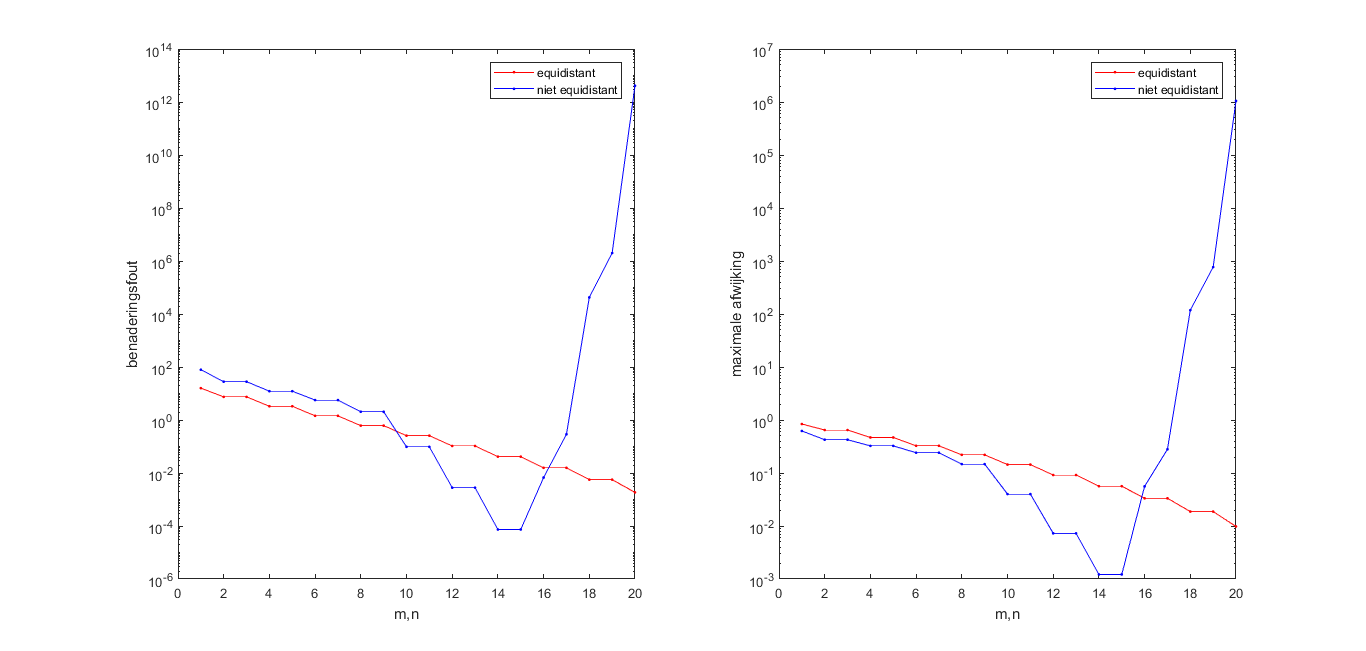
\includegraphics[width=0.8\textwidth]{oef14.png}
    \caption{benaderingsfout $\lVert f-z_{mn} \rVert_2^2$ (links) en de maximale afwijking (rechts) van de veeltermbenadering van de functie van Runge $f(x,y)=\frac{1}{1+25(x^2+y^2)}$ in functie van de graad in $x$ en $y$}
    \label{fig:oef14}
\end{figure}

